\documentclass[11pt]{article}
\usepackage[margin=1in]{geometry}
\usepackage{../../styles/isaiah}
\usepackage{fontspec}
\usepackage{bidi}
\usepackage{../../styles/components/leftRightGrid}

\begin{document}
% Isaiah Context Grid
\leftRightGrid{4}{Isaiah 6-9:7}{
    \textbf{\large Isaiah 6}

    \textit{Isaiah's Call \& \\Commission}
}{
    \textbf{\large Isaiah 7}

    \textit{Immanuel}
}{
    \textbf{\large Isaiah 8}

    \textit{Maher-shalal-hash-baz}
}
{
    \textbf{\large Isaiah 9:1-7}

    \textit{The Prince of Peace}
}

\newpage

% Main Section: Isaiah 9:1b-7
\begin{biblicaloutline}[Isaiah 9:1b-7]

    \subsectionheader{Joy Instead of Darkness (v1b-3)}
    \begin{versesection}{2em}
        \versenum{1b} In the former time he brought into contempt the land of Zebulun and the land of Naphtali, but in the latter time he has made glorious the way of the sea, the land beyond the Jordan, Galilee of the nations.
        {\vspace{1em}}
        {\versenum{2} The people who walked in \highlightsilver{darkness}}
        \poetryline{have seen a great \highlightyellow{light};}
        those who dwelt in a land of deep \highlightsilver{darkness},
        \poetryline{on them has \highlightyellow{light} shone.}

        {\versenum{3} You have multiplied the nation;}
        \poetryline{you have increased its joy;}
        {they rejoice before you}
        \poetryline{as with joy at the harvest,}
        \poetryline{as they are glad when they divide the spoil.}
    \end{versesection}

    \subsectionheader{Enemies Destroyed (v4-5)}
    \begin{versesection}{2em}
        {\versenum{4} For the yoke of his burden,}
        \poetryline{and the staff for his shoulder,}
        \poetryline{the rod of his oppressor,}
        \poetryline{you have broken as on the day of Midian.}

        {\versenum{5} For every boot of the tramping warrior} in \sectionwordfootnote{battle tumult}{Lit. "boot, booting with shaking"},
        \poetryline{and every garment rolled in blood}
        \poetryline{will be burned as fuel for the fire.}
    \end{versesection}

    \subsectionheader{Child is Born (v6-7)}
    \begin{versesection}{2em}
        {\versenum{6} For unto us a child is born,}
        \poetryline{to us a son is given;}
        {and the government shall be upon his shoulder,}
        \poetryline{and his name shall be called}
        {Wonderful Counselor, Mighty God,}
        \poetryline{Everlasting Father, Prince of Peace.}

        {\versenum{7} Of the increase of his government and of peace}
        \poetryline{there will be no end,}
        {on the throne of David and over his kingdom,}
        \poetryline{to establish it and to uphold it}
        {with \highlightaqua{justice} and with \highlightaqua{righteousness}}
        \poetryline{from this time forth and forevermore.}
        {The zeal of the LORD of hosts will do this.}
    \end{versesection}

\end{biblicaloutline}

\newpage
{\large\bfseries Matthew's Quotation of Isaiah 9:1b-2}
\vspace{1em}

Matthew 4:12-17 directly quotes this passage when describing Jesus's ministry in Galilee:

\begin{quote}
\textit{"Now when he heard that John had been arrested, he withdrew into Galilee. And leaving Nazareth he went and lived in Capernaum by the sea, in the territory of Zebulun and Naphtali, so that what was spoken by the prophet Isaiah might be fulfilled:"}\\\\
\textit{"'The land of Zebulun and the land of Naphtali, the way of the sea, beyond the Jordan, Galilee of the Gentiles— the people dwelling in darkness have seen a great light, and for those dwelling in the region and shadow of death, on them a light has dawned.'"}\\\\
\textit{"From that time Jesus began to preach, saying, 'Repent, for the kingdom of heaven is at hand.'"}\\
\hfill --- Matthew 4:12-17
\end{quote}

\vspace{1em}

So what is significant about this section of Israel in Isaiah's day, what is the significance of it in Christ's day, and why even bring up the tribal allotments from centuries earlier?
\\\\
The areas up in the north here were the first to be conquered by the Assyrians in Isaiah's day (2 Kings 15:29). They were the first wiped out, but they are also the first who are offered hope of restoration.
\\\\
And is Matthew just picking up on this because it just so happens Jesus was born in that same region? It seems Matthew is connecting not only Isaiah 9:1-2, but also a few other passages in Isaiah given his intentional change of "sitting in darkness" and "light is dawned".
\\\\
Matthew is likely pulling in Isaiah 42:1-9 which describes the Servant of the Lord who brings justice and is a light to those sitting in darkness as well as Isaiah 60:1-3 which describes the glory of the Lord rising upon Jerusalem and all nations coming to that light.
\\\\
Jesus is the servant to the nations – the glory of the Lord Himself! (who also happens to be born in that same region)


\vspace{1em}
\begin{center}

\includegraphics[width=.75\textwidth]{image.png}
\end{center}
\vspace{1em}

\newpage
{\large\bfseries The People Walking in Darkness}
\vspace{1em}

We just saw how the Northern Kingdom is explicitly called out as a people walking in darkness, but we just read in 8:14 to the end of that section that Jerusalem is also in view.
\\\\
It's a small thing, but worth noting how in Isaiah's future view of deliverance and seeing a great light, it's one unified nation (v3) of Israel, not the divided kingdoms of the past 150 years.
\\\\
God's bringing deliverance and unity to not only the nations (ch2), but also to Israel itself under the coming Child King (v6-7).

\vspace{2em}

{\large\bfseries Comparison with Judges 6-8: Gideon and the Child}
\begin{comparisontable}{}{Judges 6-8}{Isaiah 6-9:7}

\verserow{
Enemy Oppression
}{
Midianites oppressed Israel for seven years, impoverishing the land (Judg 6:1-6)
}{
Darkness and oppression over the land (Isa 8:21-22); "the yoke that burdens them" (Isa 9:4)
}

\verserow{
Divine Deliverance
}{
"The LORD is with you, mighty warrior" (gibbor) (Judg 6:12); God raises up Gideon as deliverer
}{
"His name shall be called...Mighty God" (Isa 9:6); deliverance through the Mighty (gibbor) God
}

\verserow{
Sign Requested
}{
Gideon asks for signs twice with the fleece (Judg 6:36-40)
}{
Ahaz refuses to ask for a sign; God gives the sign of Immanuel anyway (Isa 7:10-14)
}

\verserow{
"Insignificant" Leader
}{
Gideon from the weakest clan in Manasseh, least in his family (Judg 6:15)
}{
A child/infant as the deliverer (Isa 9:6); born in despised "Galilee of the Gentiles" (Isa 9:1)
}

\verserow{
Unexpected Means
}{
God reduces army from 32,000 to 300 to show His power (Judg 7:2-7)
}{
A child brings deliverance (Isa 9:6); the battle won by divine action, not human armies
}

\verserow{
Throne/Kingdom
}{
Gideon refuses kingship: "The LORD will rule over you" (Judg 8:22-23); no dynasty established
}{
"He will reign on David's throne and over his kingdom...forever" (Isa 9:7)
}

\verserow{
Weapons of War
}{
Victory achieved through unconventional weapons: trumpets, empty jars, torches (Judg 7:16-20)
}{
"Every warrior's boot...and every garment rolled in blood will be destined for burning" (Isa 9:5); end of warfare
}

\verserow{
Family Legacy
}{
Gideon's son Abimelech murders 70 brothers and becomes a tyrant (Judg 8:30-9:5); family legacy ends in violence
}{
Eternal dynasty on David's throne (Isa 9:7); names include "Everlasting Father" (Isa 9:6)
}

\end{comparisontable}

\newpage
{\large\bfseries "Prince of Peace" vs. "King"}
\vspace{1em}

Why does Isaiah use "Prince" of Peace rather than "King" of Peace?
{\hebrewword{Prince}{שַׂר}{sar}{}}

There are a few possible reasons for this choice:

\textbf{1. Assyrian Context}: Scholar R.A. Carlson suggests that \textit{sar} was deliberately chosen because it closely resembles the Assyrian word for king (\textit{sarrum}). In Isaiah's time, when Assyria dominated the ancient Near East, this linguistic connection would have communicated royal authority in terms familiar to the broader imperial context. The title may be asserting that the coming ruler would possess authority surpassing that of the Assyrian kings.

\textbf{2. Davidic Succession}: The term \textit{sar} (prince, ruler, leader) may emphasize the child as heir to the throne rather than an already-reigning monarch. Since the passage speaks of a child who is "born" and "given," the title "Prince" appropriately describes one who will ascend to royal authority. This aligns with the promise that "the government will be on his shoulders" (v6) and that he "will reign on David's throne" (v7)—future-oriented language pointing to an heir who will establish his kingdom.

\textbf{3. Military Commander}: The word \textit{sar} often carries military connotations, referring to commanders, officers, or leaders of armies (e.g., "the prince of the army" in Joshua 5:14-15). Given the context of Isaiah 9:4-5, which describes the breaking of the yoke, the rod of oppression, and the burning of military boots and bloodied garments, "Prince of Peace" may emphasize that this leader achieves peace not through endless warfare but through decisive divine victory. He is the commander who ends all wars.

\textbf{4. Poetic Sound and Rhythm}: In Hebrew, \textit{sar shalom} (\hebrew{שַׂר שָׁלוֹם}) creates an alliterative pairing with the "s/sh" sounds.

\newpage
{\large\bfseries The Pattern: Isaiah 6-9:7 and Genesis 1-12}
\vspace{1em}

The structure of Isaiah 6-9:7 follows the same redemptive pattern established in Genesis 1-12, showing that God's plan of salvation through judgment and restoration has been consistent from the beginning:

\vspace{1em}

\begin{itemize}
    \item \textbf{Creation} — Isaiah 6 opens with Isaiah's vision of God's throne room, the heavenly temple filled with glory and holiness. This establishes the divine order and God's sovereign rule over creation (like 7th day).

    \item \textbf{A Testing (often involving food)} — Isaiah 7 presents King Ahaz with a test: will he trust God or seek alliance with Assyria? God offers him a sign, any sign he wants, to confirm His promise.

    \item \textbf{Moral Failings} — Ahaz refuses to ask for a sign (Isaiah 7:12), rejecting God's offer. This represents the failure of God's people to trust Him, paralleling Adam and Eve's failure in the garden. The sin continues spiraling.

    \item \textbf{Flood of Judgment} — Isaiah 8:5-8 depicts the Assyrian invasion as a flood that will "sweep on into Judah, it will overflow and pass on, reaching even to the neck." The waters of judgment come upon the land.

    \item \textbf{Decreation} — Isaiah 8:19-22 describes the land returning to chaos: "distressed and hungry...darkness and gloom, the distress of anguish...thrust into thick darkness."

    \item \textbf{Righteous, Faithful Intercessor} — The promised child of Isaiah 7:14 (Immanuel) and 9:6-7 serves as the faithful one where Ahaz failed. Unlike Adam who brought death, this child brings life and establishes an eternal kingdom.

    \item \textbf{New Creation} — Isaiah 9:1-7 bursts forth with new creation language: light shining in darkness, joy and abundance replacing mourning, weapons of war burned, and the government resting on the shoulders of the Prince of Peace who reigns forever.
\end{itemize}

\newpage

\begin{center}
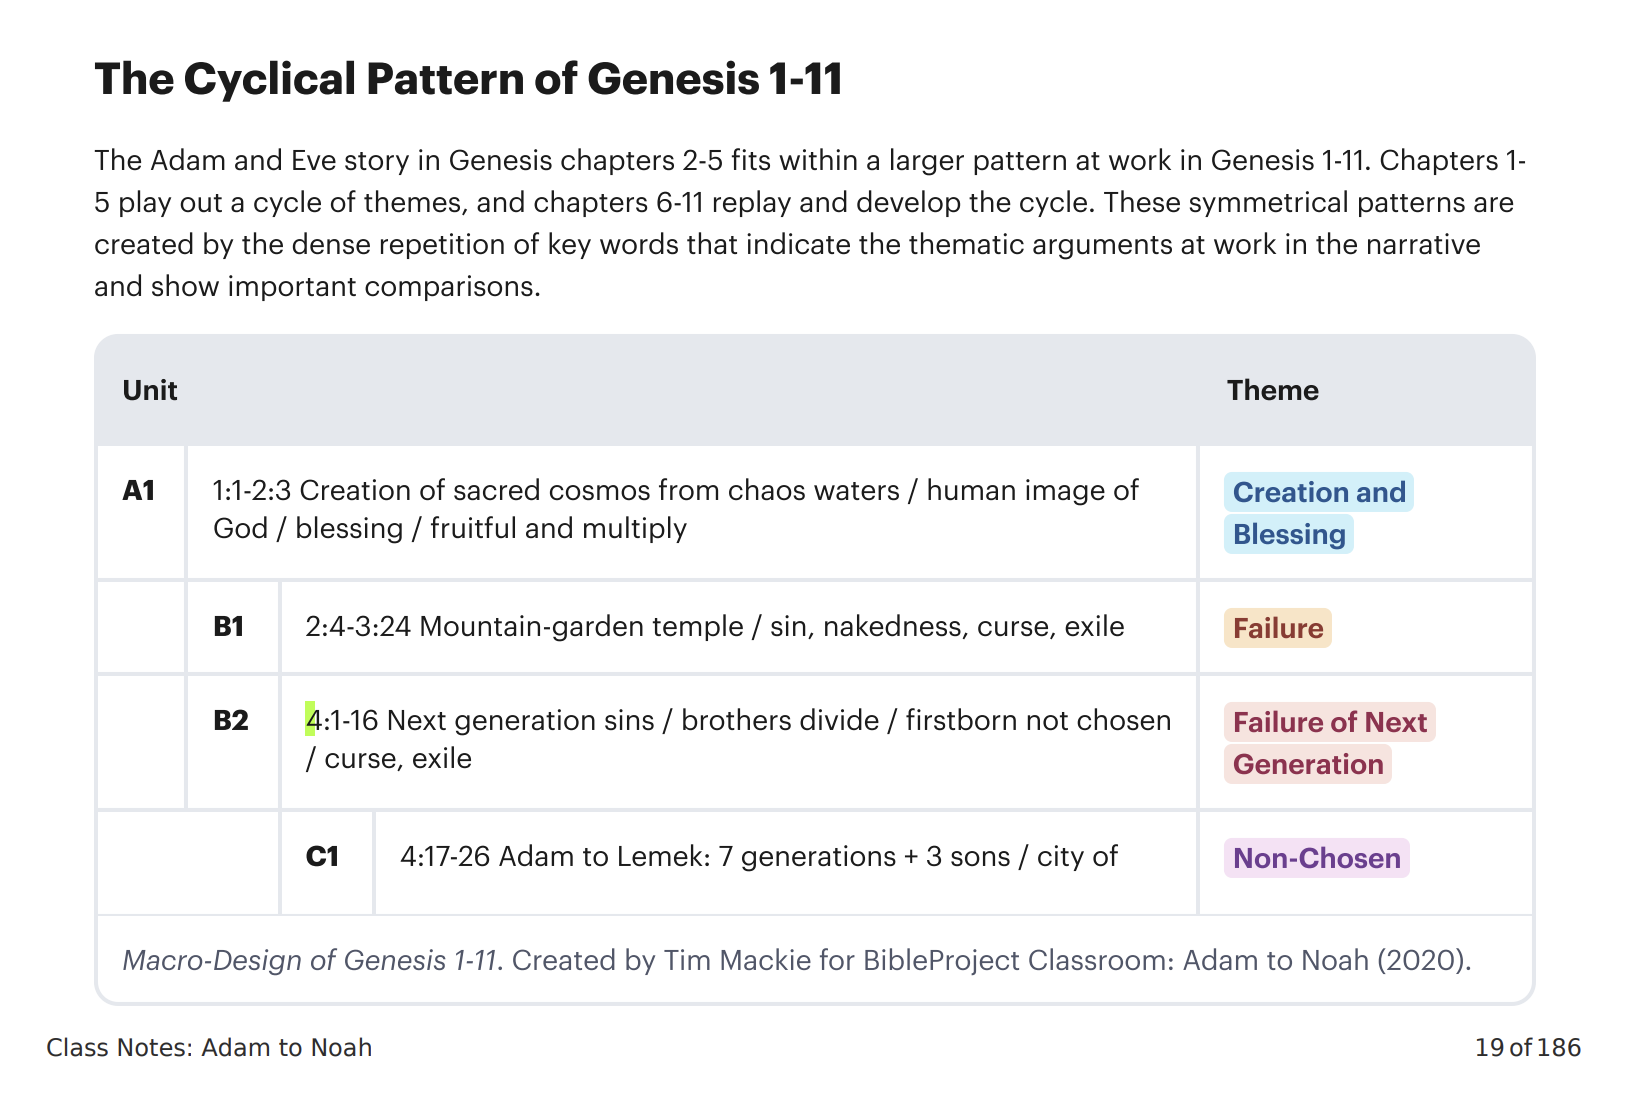
\includegraphics[width=.86\textwidth]{table1.png}
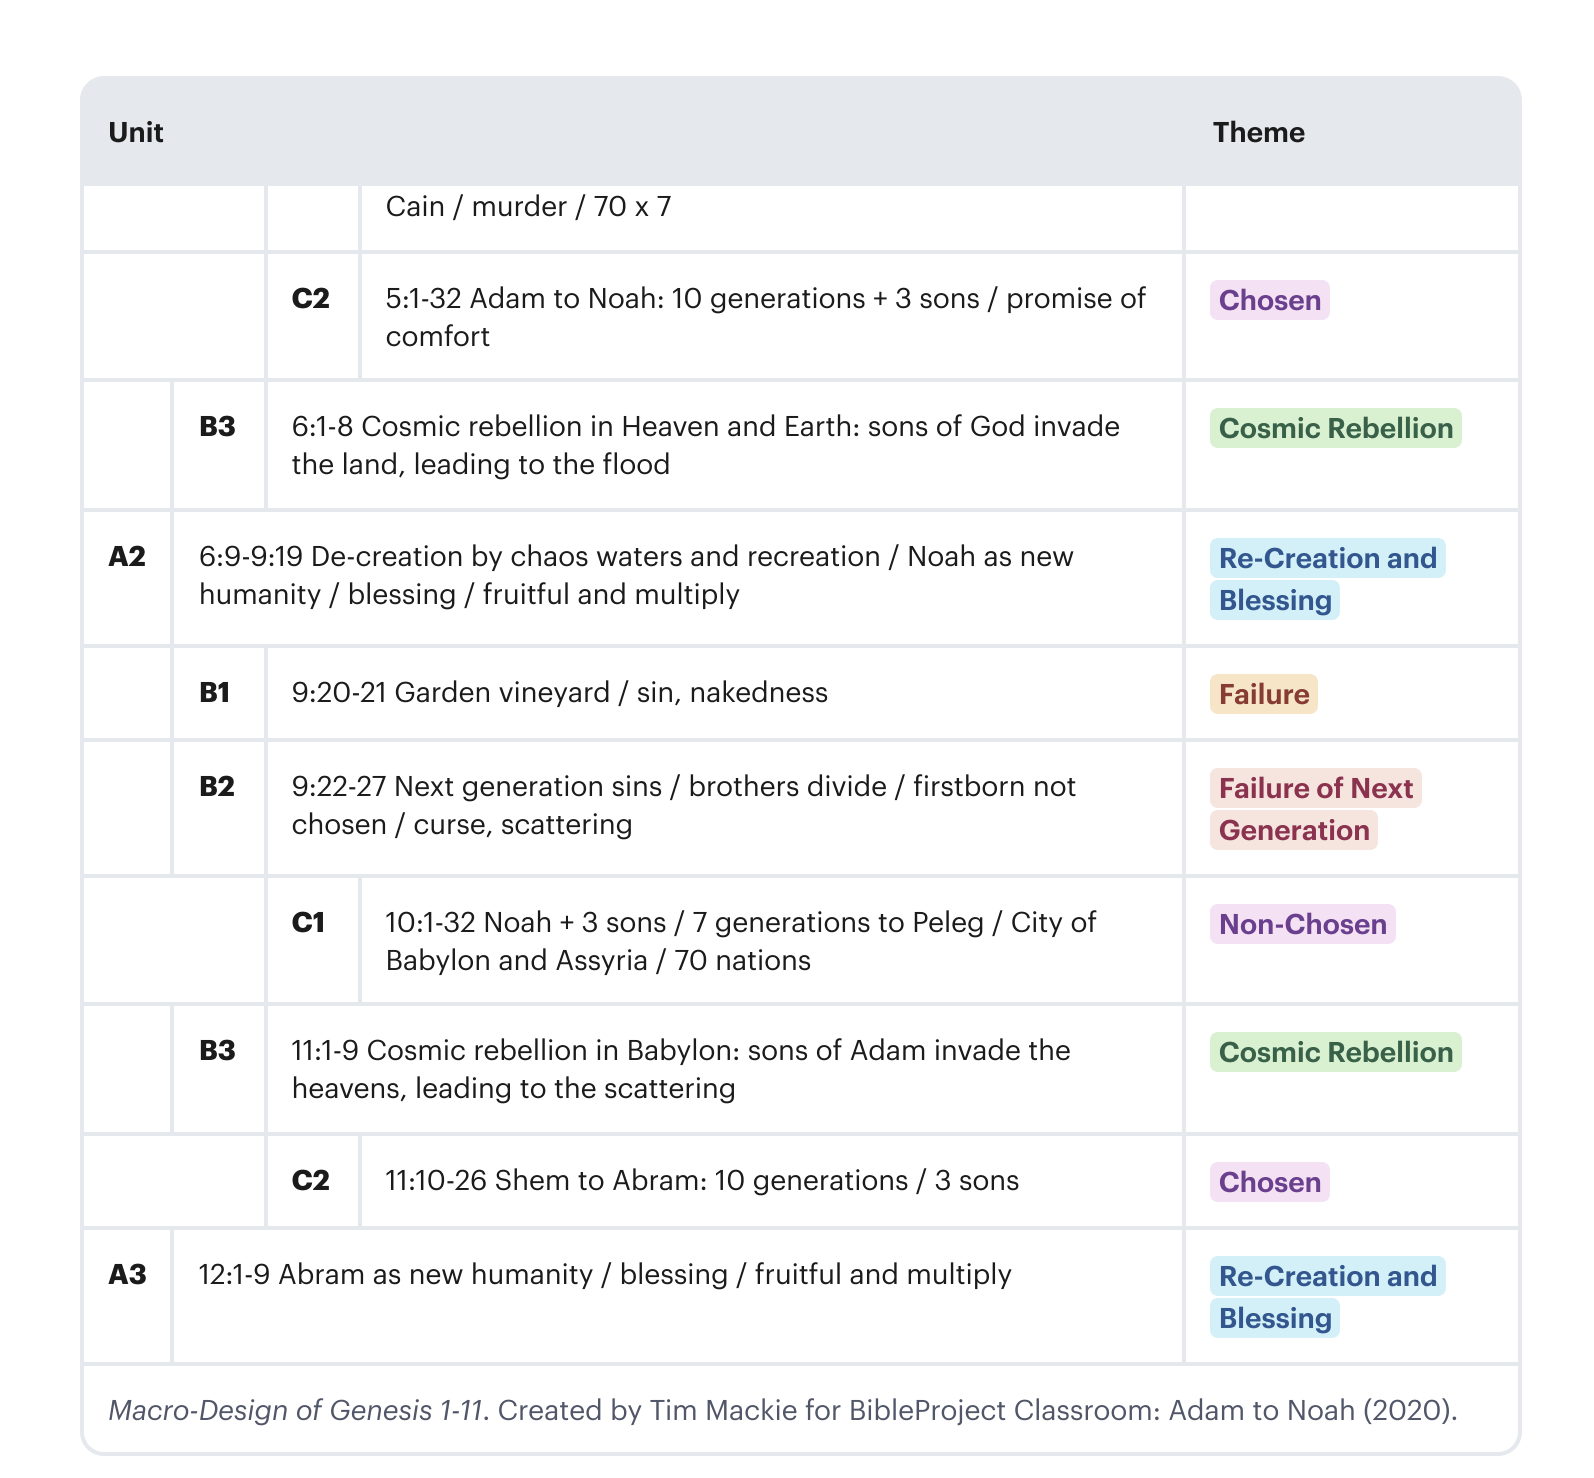
\includegraphics[width=.86\textwidth]{table2.png}
\end{center}

\end{document}